%%%%%%%%%%%%%%%%%%%%%%%%%%%%%%%%%%%%%%%%%%%%%%%%%%%%%%%%%%%%%%%%%%%%%%%%%%%
%%%                                                                     %%%
%%%   LaTeX template voor het verslag van P&O: Computerwetenschappen.   %%%
%%%                                                                     %%%
%%%   Opties:                                                           %%%
%%%     tt1     Tussentijdsverslag 1                                    %%%
%%%     tt2     Tussentijdsverslag 2                                    %%%
%%%     tt3     Tussentijdsverslag 3                                    %%%
%%%     eind    Eindverslag                                             %%%
%%%                                                                     %%%
%%%   2 oktober 2012                                                    %%%
%%%   Versie 1.0                                                        %%%
%%%                                                                     %%%
%%%%%%%%%%%%%%%%%%%%%%%%%%%%%%%%%%%%%%%%%%%%%%%%%%%%%%%%%%%%%%%%%%%%%%%%%%%

\documentclass[tt1]{penoverslag}

%%% PACKAGES
\usepackage{lipsum}
\usepackage{gensymb}
\usepackage [dutch] {babel}
\usepackage{graphicx}
\usepackage{amsmath}
\usepackage{fullpage}
\usepackage{listings}

\begin{document}

% == VOORPAGINA == %
\team{Zilver} % teamkleur
\members{Sam Gielis\\
         Sophie Marien\\
         Toon Nolten\\
         Nele Rober\\
         Gerlinde Van Roey\\
         Maxim Van Mechelen} % teamleden

\maketitlepage

% == ABSTRACT EN INHOUDSTAFEL == %
\begin{abstract}
\label{ssec:abstr}
De robot wordt voor demo 1 nog niet voorzien van sensoren. De focus ligt vooral op de nauwkeurigheid van de besturing en op het implementeren van alle softwarecomponenten. Deze software bestaat uit twee projecten: een op de computer en een op de robot. De computersoftware bestaat uit een Grafical User Interface (GUI), enkele Communication klassen die informatie doorsturen en enkele klassen die de werking van de robot simuleren (simulator).
\end{abstract}

\tableofcontents

%figuur robot
\begin{figure}[!b]
\begin{flushright}
    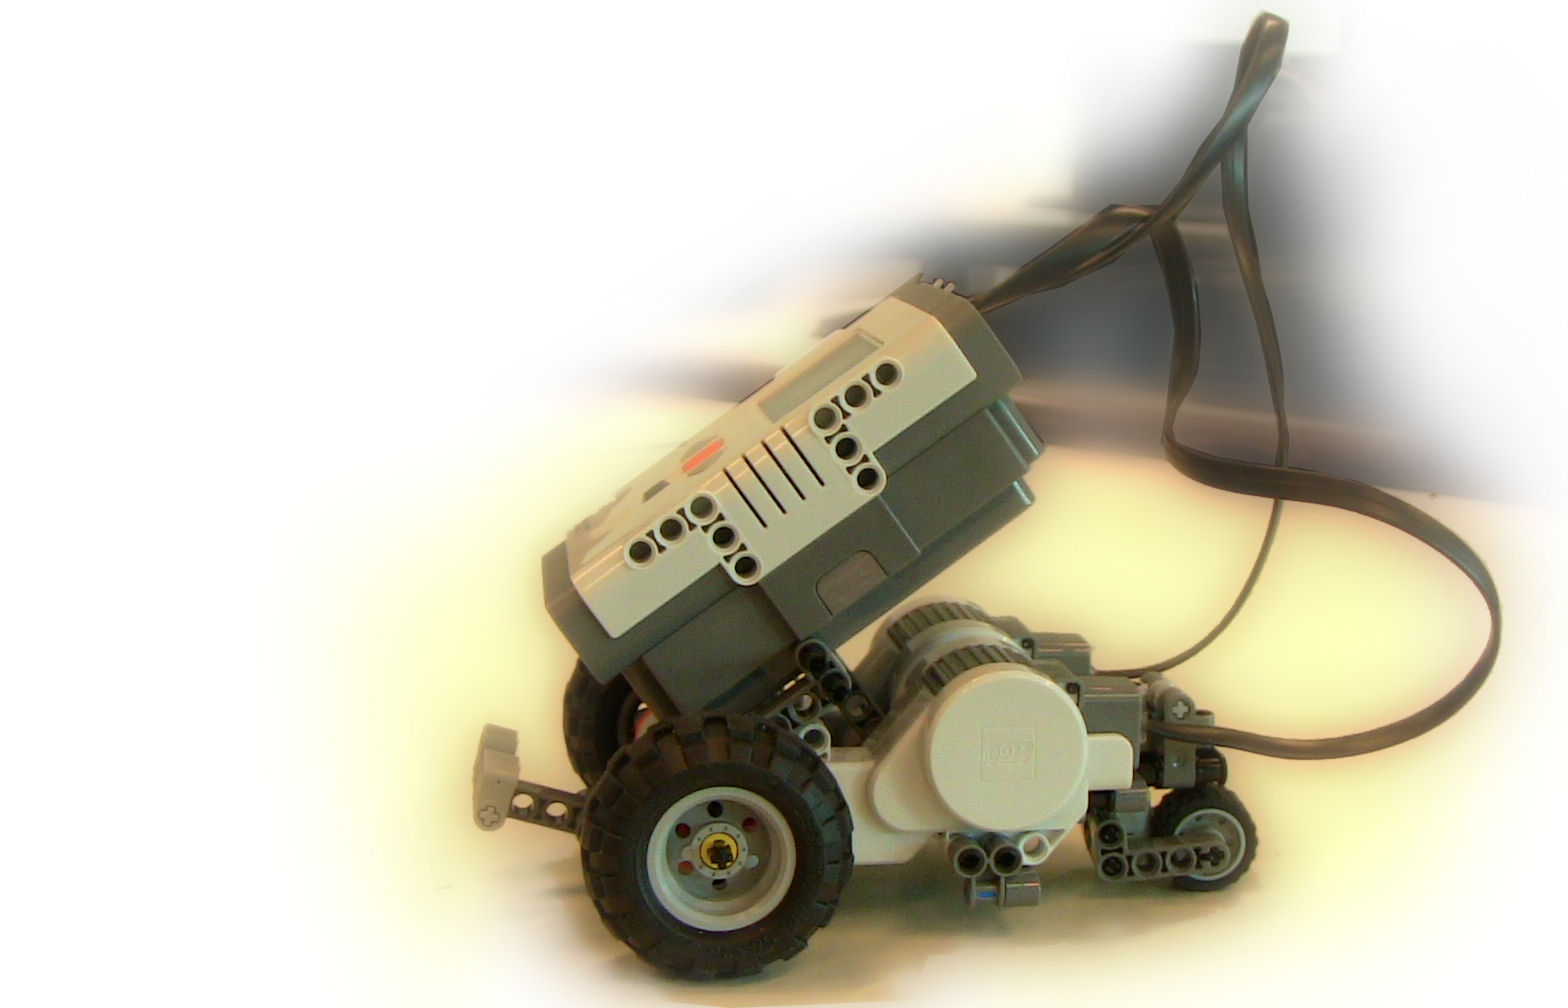
\includegraphics[width=1\textwidth]{robotFP2}
	\label{fig:robotFP}
\end{flushright}
\end{figure}


\newpage

% == INLEIDING == %
\section{Inleiding}
\label{ssec:inl}
In het kader van het vak 'Probleemoplossen en Ontwerpen: computerwetenschappen' wordt gewerkt rond autonome intelligente robots. Verschillende teams bouwen en programmeren een robot met behulp van LEGO Mindstorms. Deze robot moet uiteindelijk volledig autonoom een doolhof kunnen verkennen.
Op de eerste demonstratie verbindt de robot via bluetooth met de computer. De GUI laat toe de robot via pijltjestoetsen handmatig te besturen of een veelhoek te rijden. De parameters voor deze veelhoek, het aantal hoeken en de lengte van de zijde, kunnen via de GUI ingegeven worden. Een simulator is in staat dezelfde demonstratie te tonen.

% == BOUW == %
\section{Bouw van de robot}
\label{ssec:bouw}
LEGO Mindstorms\footnote{\textit{Lego Mindstorms}:  Een uitbreiding op de LEGO bouwstenen waarmee kleine, aanpasbare en programmeerbare robots gebouwd kunnen worden. Een centrale besturingsmodule ('the brick') kan geprogrammeerd worden met verschillende programmeertalen. In eerdere versies werd een RCX gebruikt voor de brick, nu wordt met NXT gewerkt. De brick kan enkele motoren aandrijven. Bovendien kunnen er verschillende sensoren, o.a. een druksensor en een lichtsensor, aangesloten worden.  \mbox{[www.lego.com]} \mbox{[http://en.wikipedia.org/wiki/Lego\textendash Mindstorms]}} biedt een bouwpakket voor een robot aan. Een NXT-microcomputer laat toe de robot te programmeren met Java.

% == fysieke bouw == %
\subsection{Fysieke bouw}
\label{ssec:fysbouw}
Bij het bouwen van de robot (zie figuur \ref{robot}) werd het ontwerpboekje gevolgd dat bij het bouwpakket geleverd zat. Deze compacte samenstelling leek geen directe nadelen te hebben.
Eerst zijn alle sensoren op de robot geplaatst. De lichtsensor vooraan, zo dicht mogelijk tegen de grond om zo goed mogelijk te kunnen lezen. De druksensor erboven, zodat een botsing kan worden waargenomen. De ultrasonesensor bovenaan, als een hoofd, om een breed 'gezichtsveld' te hebben. Uiteindelijk hebben we beslist de sensoren voorlopig nog niet aan te sluiten, omdat deze voor de eerste demonstratie nog niet nodig zijn.

%figuur robot
\begin{figure}[tbp]
\begin{center}
    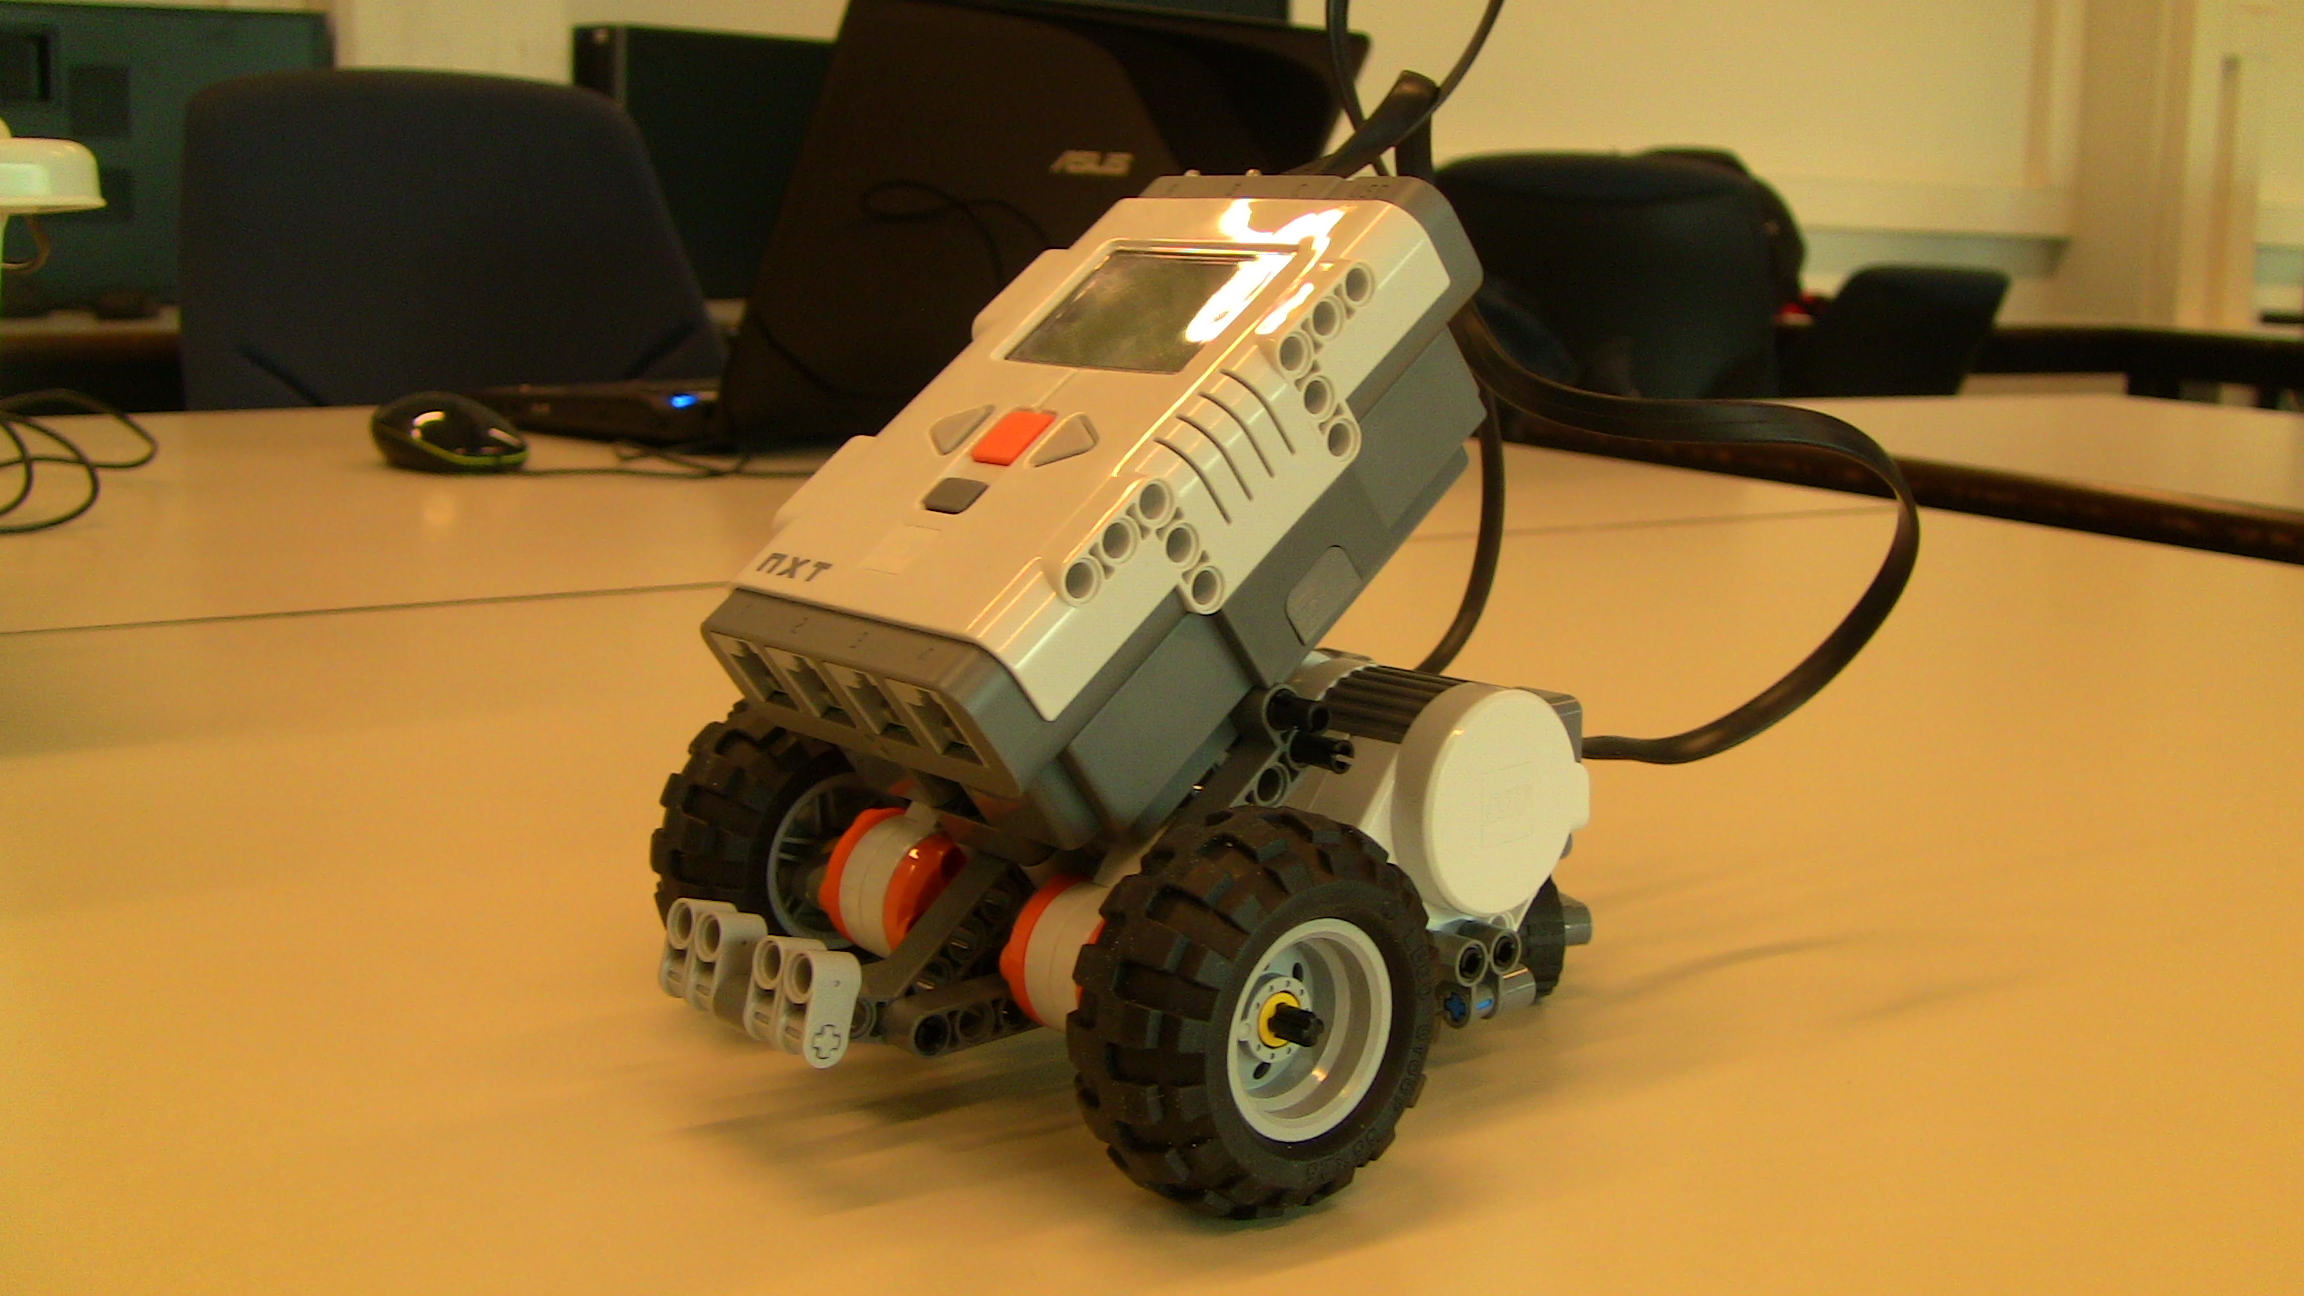
\includegraphics[width=0.8\textwidth]{robot}
    \caption{Robot}
	\label{robot}
\end{center}
\end{figure}

% == calibratie == %
\subsection{Calibratie}
\label{ssec:calib}
Door de diameter van het wiel op te meten, kan geschat worden hoeveel graden een wiel rond zijn as moet draaien om \'e\'en centimeter vooruit te komen. Om een exactere waarde van deze parameter te bekomen, werd verder via 'trial-and-error' gewerkt. Dit gebeurde door de robot naast een lintmeter precies \'e\'en meter af te laten leggen en de parameter aan te passen waar nodig. Het resultaat werd door 100 gedeeld.
Ter controle van het bekomen resultaat werden ook andere afstanden getest.
Om de robot om zijn as te laten draaien, bewegen beide wielen in tegengestelde richting. De robot werd naast een lijn geplaatst. De parameter werd aangepast tot de robot na het draaien opnieuw precies naast de lijn uitkwam.
De resultaten van de calibratie worden weergegeven in tabel \ref{tab:meetresult}.

%overzicht meetwaarden
\begin{table}[tbp]
\begin{center}
    \begin{tabular}{ | l | l | l | l |}
    \hline
     & linkerwiel & rechterwiel & aantal graden \\ \hline
    1 cm vooruit & voor & voor & 20,8\degree
    \\ \hline
    1 cm achteruit & achter & achter & 20,8\degree
    \\ \hline
    180\degree draaien linkssom & achter & linker & 701\degree \\ \hline
    180\degree draaien rechtsom & voor & achter & 701\degree \\ \hline
    \end{tabular}
	\caption{Resultaten calibratie}
    \label{tab:meetresult}
\end{center}
\end{table}

% == SOFTWARE == %
\section{Software}
\label{sec:softw}
De software bestaat uit twee delen: een project dat op de NXT van de robot loopt en een project dat op de computer loopt. Alles wordt aangestuurd via de Graphical User Interface (GUI). Deze toepassing laat toe de robot te besturen (via bluetooth) en de reacties van de robot te simuleren met de simulator. Een Communication-pakket stuurt de commando's van de GUI door naar de juiste unit.
De simulator kan gebruikt worden om de software op te testen zonder telkens op de robot te moeten wachten.

% == software design == %
\subsection{Software ontwerp}
\label{ssec:Sdesign}
Zoals reeds vermeld bestaat de software uit twee projecten: \'e\'en draait op een computer en \'e\'en draait op de NXT-Brick. Figuren \ref{fig:klasDiaPC} en \ref{fig:klasDiaNXT} tonen een klassendiagram van de projecten.\\
Beide projecten hebben een identiek package \textit{commands} met \'e\'en klasse \textit{Command}. Hierin staan de final static integers die met de mogelijke bluetoothsignalen overeenkomen (zie sectie \ref{ssec:commands}). Een verdere beschrijving van de software op de NXT-brick wordt in sectie \ref{ssec:robot} gegeven.\\
Het computerproject heeft nog drie andere packages: \textit{communication}, \textit{gui} en \textit{simulator}. Het package \textit{gui} heeft enkel de klasse \textit{SilverSurferGUI} die de functionaliteit van de GUI implementeert (zie sectie \ref{ssec:GUI}). De GUI communiceert met de simulator of de robot via de klassen in het package \textit{communication} door een object van de superklasse \textit{UnitCommunicator} bij te houden. Aan deze \textit{UnitCommunicator} is een object van de subklassen \textit{RobotCommunicator} of \textit{SimulatorCommunicator}  toegekend. Zo worden de commands dynamisch naar de juiste unit gestuurd. De \textit{RobotCommunicator} communiceert met het NXT-Project, de \textit{SimulatorCommunicator} met de simulator klassen. Het package \textit{simulator} tenslotte, implementeert de functionaliteit van de simulator zoals beschreven in sectie \ref{ssec:simulator}.


%figuur klassendiagram PC
\begin{figure}[tbp]
\begin{center}
    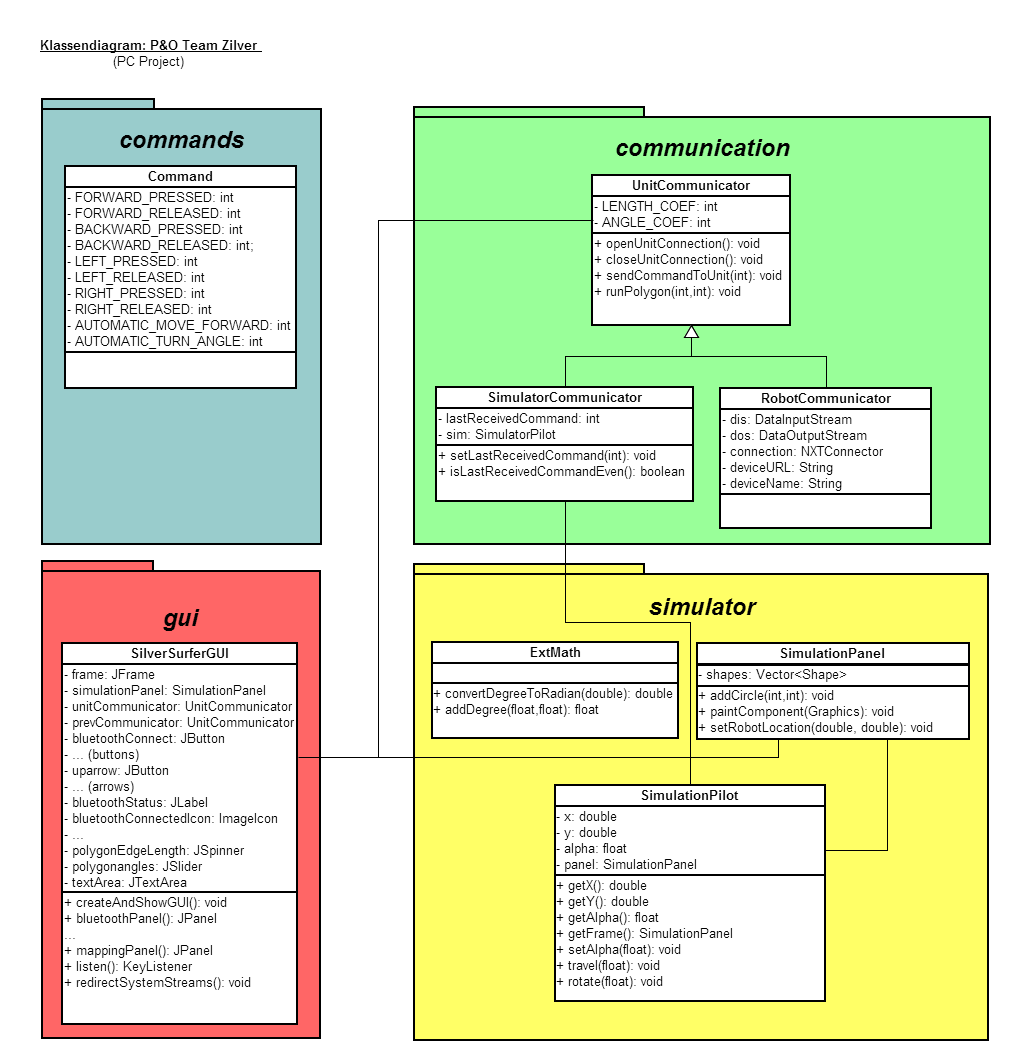
\includegraphics[width=0.8\textwidth]{KlassendiagramPC}
    \caption{Klassendiagram van de software die op de PC loopt}
	\label{fig:klasDiaPC}
\end{center}
\end{figure}

%figuur klassendiagram NXT
\begin{figure}[tbp]
\begin{center}
    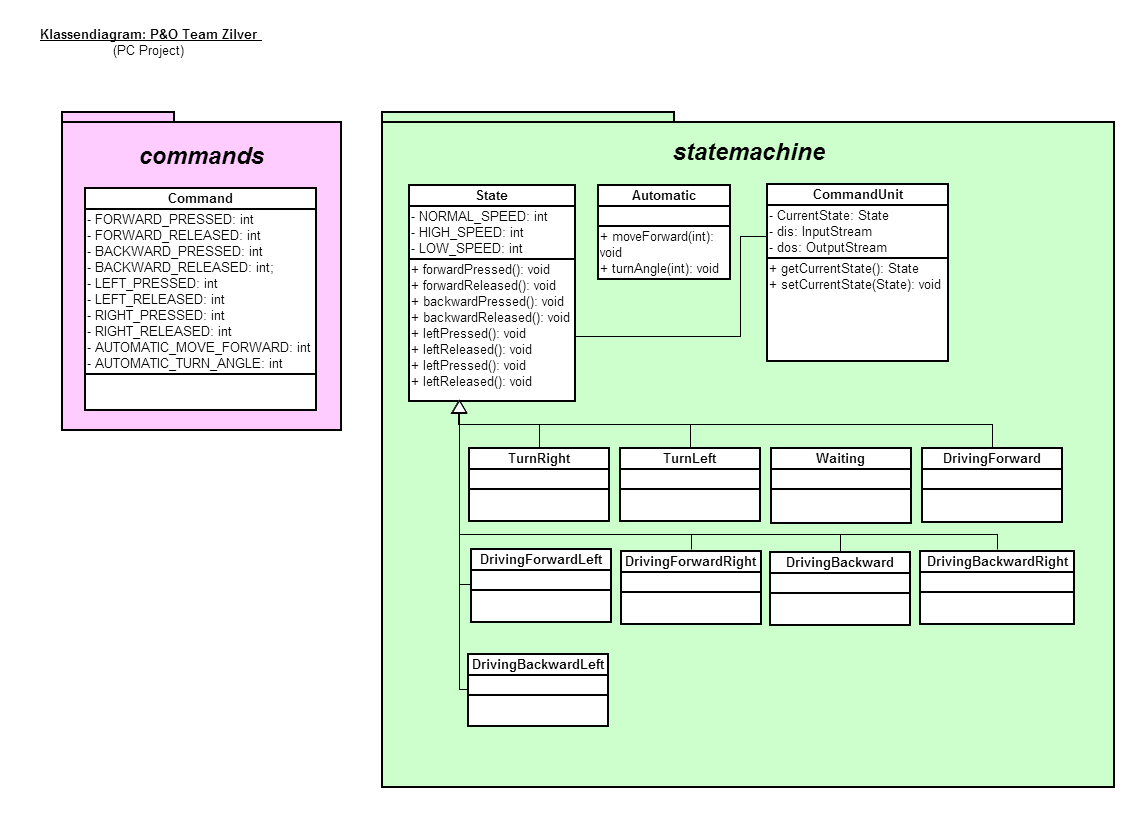
\includegraphics[width=0.8\textwidth]{KlassendiagramNXT}
    \caption{Klassendiagram van de software die op de robot loopt}
	\label{fig:klasDiaNXT}
\end{center}
\end{figure}

% == commando's == %
\subsection{Het doorgeven van commando's}
\label{ssec:commands}
De GUI zet een actie van de gebruiker om in een commando. Dit commando wordt gerepresenteerd door een integer, zoals reeds in sectie \ref{ssec:Sdesign} werd vermeld, dat naar de \textit{UnitCommunicator} wordt gestuurd. Twee van de commando's hebben echter extra informatie nodig: \textit{automatic move x cm forward} en \textit{rotate x degrees}. Deze informatie wordt toegevoegd aan de integer door de integer uit te breiden met extra cijfers (dit wordt in sectie \ref{sssec:integer} in detail beschreven).\\
De \textit{UnitCommunicator} stuurt de bekomen integer door naar ofwel de \textit{RobotCommunicator} ofwel de \textit{SimulatorCommunicator}. Deze zetten de integer weer om in de juiste actie van respectievelijk de robot en de simulator. De wijze waarop dit gebeurt verschilt licht voor beide gevallen. Zo stuurt de \textit{RobotCommunicator} zijn commando's via Bluetooth door naar de NXT-brick, terwijl de \textit{SimulatorCommunicator} zo'n verbinding niet nodig heeft.\\

\subsubsection{De bewerking op de integers}
\label{sssec:integer}
Integers stellen de commando's voor. In twee gevallen is echter meer informatie nodig: om de robot een bepaalde afstand af te laten leggen en om de robot een bepaald aantal graden te laten draaien. Deze afstand en dit aantal graden moet mee doorgegeven worden in de vorm van een integer. De eenheden waarin de afstand en hoek worden doorgestuurd zijn respectievelijk cm en graden.\\\\
De doorgegeven integer wordt als volgt opgebouwd:

\begin{itemize}
\item de waarde van de afstand (hoek) wordt vermenigvuldigd met 1000.
\item de integer die het commando representeert, wordt hierbij opgeteld.
\end{itemize}

Om de bekomen resultaten terug op te splitsen in de twee oorspronkelijke gegevens worden volgende stappen gevolgd:

\begin{itemize}
\item een modulo-operatie van tien geeft het laatste cijfer terug. Dit stelt het soort commando voor.
\item dit getal wordt van de integer terug afgetrokken.
\item de oorspronkelijke afstand (hoek) wordt bekomen door de integer door 1000 te delen.
\end{itemize}

Deze werkwijze brengt een beperking met zich mee: de waarde van de afstand (hoek) kan slechts tot 2 cijfer(s) na de komma doorgegeven worden. De robot kan niet nauwkeuriger dan 0,1 cm aangestuurd worden. Hierdoor is het niet nodig de afstand nauwkeuriger door te geven. De veelhoek stapelt echter veel afrondingsfouten op naarmate de lengte van de zijde en/of het aantal hoeken stijgt. Het valt op als de som van de berekende hoeken geen 360 graden is: begin- en eindpunt vallen dan niet samen. 

% == gui == %
\subsection{GUI}
\label{ssec:GUI}
De GUI bestaat uit twee vensters, enkele knoppen en enkele instelmogelijkheden: zie figuur \ref{fig:gui}. Deze knoppen besturen ofwel de robot ofwel de simulator, naargelang de bluetooth verbinding aan staat. In deze sectie wordt verder enkel de robot vermeld. Dezelfde functionaliteiten gelden echter ook voor de simulator.

%overzicht functionaliteiten
\begin{itemize}
\item \textit{onderste venster:} debuginformatie van de robot.
\item \textit{bovenste venster:} tekent de baan van de robot. In latere demo's geeft dit venster ook de doolhof weer.
\item \textit{bluetooth connectieknop:} zet de verbinding op of af. Het icoontje ernaast verandert naargelang de status van de verbinding.
\item \textit{veelhoekinstellingen:} stellen de parameters van de veelhoek in. De knop doet de robot de veelhoek effectief rijden.
\item \textit{pijltjestoetsen:} besturen de robot manueel.
\end{itemize}

Twee parameters bepalen de veelhoek die de robot rijdt: het aantal hoeken van de figuur en de lengte van de zijden.
Een JSlider laat toe het aantal hoeken in te geven. Dit geeft de mogelijkheden overzichtelijk weer. Bovendien kan zo het bereik beperkt worden tot 30. Bij een groter aantal hoeken, streeft een veelhoek immers naar een cirkel.
Het bereik van de lengte van de zijden is groter: van \'e\'en centimeter tot een onbeperkte grootte. Hierdoor is het een betere optie om voor JSpinner te kiezen. 

%figuur gui
\begin{figure}[tbp]
\begin{center}
    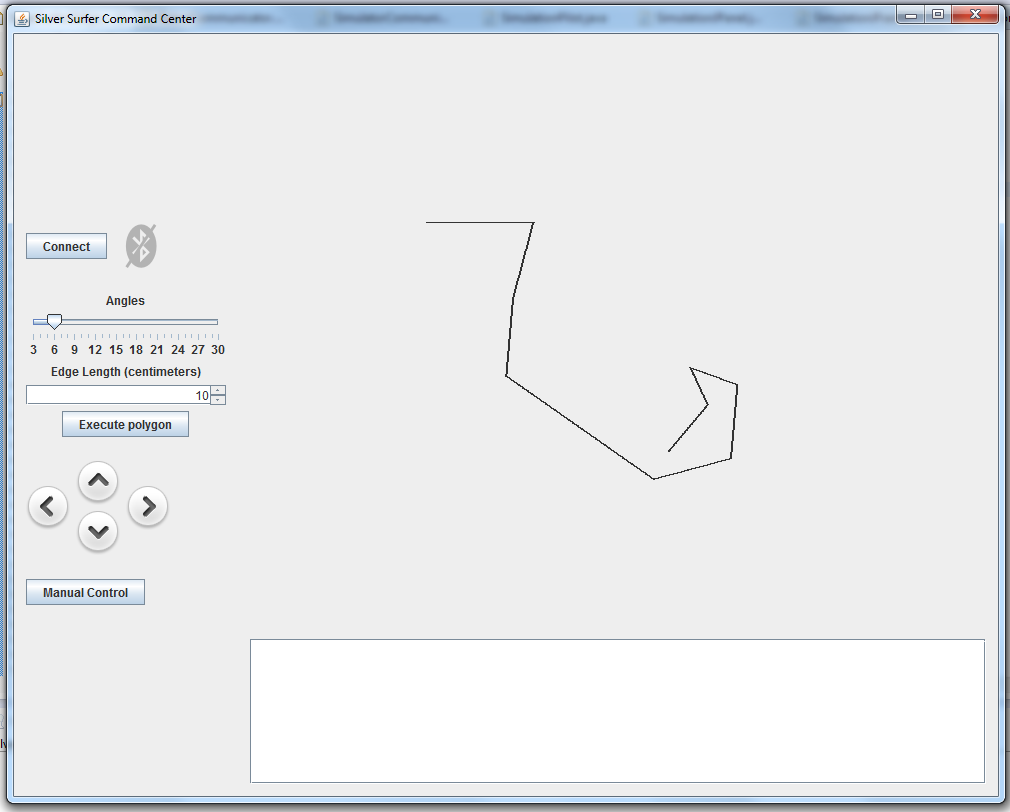
\includegraphics[width=0.8\textwidth]{GUI}
    \caption{Grafische User Interface}
	\label{fig:gui}
\end{center}
\end{figure}

% == bluetooth == %
\subsection{Bluetooth}
\label{ssec:bluetooth}
De communicatie tussen robot en computer gebeurt volledig via bluetooth. De GUI voorziet een knop om deze verbinding te maken en geeft de status van de verbinding weer. De GUI stuurt commando's door naar de robot via de klassen \textit{UnitCommunicator} en \textit{RobotCommunicator}.

De leJOS-API\footnote{\textit{leJOS}:  Een kleine Java Virtuele Machine die toelaat de NXT-brick te programmeren. leJOS voorziet verschillende klassen die o.a. de motoren aansturen en een bluetoothverbinding opzetten.  \mbox{[http://lejos.sourceforge.net/]}} voorziet de \textit{NXTConnector} klasse. De methode \textit{connectTo((String, String, int, int)} zet de bluetoothverbinding tussen computer en brick op. De belangrijkste argumenten hiervoor zijn de naam van de NXT-Brick en zijn DeviceUrl  - in het geval van de gebruikte NXT: 'Silver' en '00:16:53:0A:04:5A'.

% == robot == %
\subsection{Robot}
\label{ssec:robot}
Een \textit{Finite State Machine} geeft de robot een concreet uitvoeringsschema. Dit is als volgt ge\"implementeerd (zie figuur \ref{fig:klasDiaNXT}): een object van de klasse \textit{CommandUnit} houdt een currentState bij - een object van de superklasse \textit{State}. Negen subklassen verzorgen het nodige onderscheid: \textit{Waiting}, \textit{DrivingBackward}, \textit{TurnLeft}, \textit{DrivingRightForward}, …  en \'e\'en speciale toestand: de klasse \textit{Automatic}. De \textit{CommandUnit} ontvangt commando's via bluetooth. De \textit{CommandUnit} wijzigt de currentState naar een nieuw object van een \textit{State}-subklasse. De constructoren van elke subklasse passen het gedrag van de motoren aan bij de overgang naar de bepaalde state.
Bijvoorbeeld: De robot staat stil en zijn currentState is \textit{Waiting}.
Als de gebruiker de robot voorwaarts wil laten gaan, drukt hij de up-toets in. De \textit{CommandUnit} wijzigt de currentState van de robot naar currentState.ForwardPressed(). Dit levert een currentState van het type \textit{DrivingForward} op. De robot beweegt voorwaarts.
Tot slot is er de klasse \textit{Automatic}. Deze heeft twee methoden: \textit{turnAngle(int)} en \textit{driveForward(int)}. De \textit{CommandUnit} roept deze methoden op met argumenten die hij geparsed heeft uit de informatie van de ontvangen signalen, zoals beschreven in sectie \ref{ssec:commands}.

% == simulator == %
\subsection{Simulator}
\label{ssec:simulator}
De simulator bootst de werking van de robot virtueel na. Hij kan dezelfde commando's uitvoeren als de werkelijke robot. De GUI stuurt de simulator aan via de klassen \textit{UnitCommunicator} en \textit{SimulatorCommunicator}. Deze ontvangen de uit te voeren commando's, analyseren ze en sturen ze door naar de simulator.
\\
De simulator zelf bestaat uit vier klassen:

%overzicht klassen simulator
\begin{itemize}
\item \textit{SimulationJFrame:} zet het tekenpaneel op.
\item \textit{SimulationPanel:} tekent de baan van de 'robot' in het tekenpaneel.
\item \textit{ExtMath:} doet enkele berekeningen.
\item \textit{SimulationPilot:} houdt de positie en de richting van de 'robot' bij.
\end{itemize}

Wanneer de 'robot' een pad aflegt, tekent de simulator dit in het tekenpaneel als een zwarte lijn (herschaald: \'e\'en cm = \'e\'en pixels). De lijn  bestaat uit verschillende cirkels die elkaar gedeeltelijk overlappen. Het \textit{SimulationPanel} houdt alle bezochte co\"ordinaten bij. De klasse bevat een methode die deze cirkels \'e\'en na \'e\'en tekent. Dit zorgt ervoor dat de lijn continu bijgewerkt wordt.

De simulator begint te tekenen na het krijgen van een commando.



% == BESLUIT == %
\section{Besluit}
De uiteindelijke fysieke bouw van de robot bestaat uit de NXT en de wielen met aandrijvingen. Alle sensoren werden voorlopig weggelaten. 
De calibratie van de robot zorgt ervoor dat hij precies aangestuurd kan worden.
De GUI gebruikt een eenvoudige interface en bevat knoppen waarmee de robot handmatig bestuurd kan worden. Door het ingeven van parameters in de GUI kan de robot een willekeurige veelhoek rijden. De simulator is ook verbonden aan de GUI. Deze voert dezelfde opdracht uit als de robot. De simulator is handig om testen op uit te voeren, zonder steeds op de robot te moeten wachten.

\end{document}
